\section{Лекция 1}
\subsection{Пример}

\begin{wrapfigure}{l}{0.17\linewidth}
    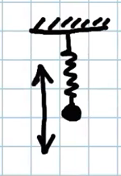
\includegraphics[width=\linewidth]{images/pendulum.png}
\end{wrapfigure}
Вспомним модель математического маятника. Каким образом дифференциальные уравнения, в зависимости от разной степени точности модели могут характеризовать конкретную ситуацию?

Пусть $y(t)$ - координата шарика. В случае идеальной системы, для описания поведения координаты в зависимости от времени у нас имеется следующее уравнение:  $$\ddot{y} + w^2y = 0$$Решением этого уравнения будет семейство функций следующего рода: $$y=a\cdot sin(wt+\varphi_0)$$, где $\varphi_0$ и $a$ произвольные постоянные, которые зависят от конкретной ситуации. Обратите внимание: количество произвольных констант совпадает с порядком производной.
\textbf{Важно помнить об общей закономерности количества произвольных констант и порядком старшей производной.}

В ситуации, когда присутствует сопротивление среды уравнение, описывающее систему, примет вид:
$$\ddot{y} + 2 \beta \dot{y} +w^2y = 0$$
Откуда следует, что
$$y=a e^{-\beta t}sin( \widetilde{w}t +\varphi_0)$$
$$\widetilde{w}=\sqrt{w^2-\beta^2}$$

\subsection{Постановка задачи}
Пусть функция $y(x)$ определенна вместе с $n$ своими производными на некотором премежутке $I$ (промежутком $I$ называется такое подмножество действительной оси, что для любых различных $x_1$ и $x_2$ принадлежащих этому промежутку, ему будет принадлежать и весь интервал $(x_1, x_2) \subset I$. Промежутками является сама прямая, лучи, отрезки, интервалы, полуинтервалы).

Пусть функция нескольких переменных $F(x,y,p_1,\ldots,p_n)$ определена и непрерывна на некотором подмножестве действительного пространства $\Omega \subset \mathbb{R}^{n+2}$. С помощью этих величин введем определение дифференциального уравнения $n$-го порядка.

\begin{Def}
Уравнение вида
\begin{equation}\label{1}
    F(x, y, y', \ldots, y^{(n)}) = 0
\end{equation}
называется обыкновенным дифференциальным уравнением $n$-го порядка.
\end{Def}
\begin{Def}
Функция $\varphi(x)$, определенная на $I$ вместе со своими $n$ производными, называтся решением уравнения (\ref{1}), если
\begin{enumerate}
    \item $\varphi$ и её $n$ производных непрерывны на $I$
    \item $\forall x \in I$ $(x, \varphi(x), \varphi'(x), \ldots, \varphi^{(n)}(x)) \in \Omega$
    \item $\forall x \in I$ $F(x, \varphi(x), \varphi'(x), \ldots, \varphi^{(n)}(x))=0$
\end{enumerate}
\end{Def}

\subsection{Простейшие уравнения 1-го порядка}
\begin{Def}
Уравнение вида $y'=f(x,y)$ называется уравнением, разрешенным относительно производной.
\end{Def}
\begin{Def}
Уравнение вида $P(x,y)dx +Q(x,y)dy=0$ называется уравнением в дифференциалах. Откуда можно выразить:
$$y_x'=-\frac{P(x,y)}{Q(x,y)}\;\;\;\;\;\;\;\; x_y'=-\frac{Q(x,y)}{P(x,y)}$$
\end{Def}
\subsubsection{Уравнения с разделяющимися переменными}
\begin{enumerate}
    \item $y'=f(x)g(y)$ ($f(x)$ непрерывна на $I_1$, $g(y)$ непрерывна на $I_2$)
    \begin{nonum}
    Решим $g(y)=0$. Пусть $g(y_k)=0$, $y_k \in I_2$, $k=\overline{1,n}$. В таком случае $g(y_k)$ обращается в 0, и производная от константы также 0. Важно, что количество $y_k$ должно быть конечно: так как мы работаем на ограниченном промежутке $I_2$, более чем конечное число нулей может означать, что мы не сможем организовать между этими нулями промежутки, определенной положительной длины, на которых $g$ принимает значения одного и того же знака. Если мы берем более чем конечное множество на ограниченом промежутке, то получаем предельную точку. Соответсвенно нам не удастся отыскать промежутки знакопостоянства $g(y)$.
    
    Тогда $y\equiv y_k$ - решения уравнения.
    Дальше, там где $g(y)$ в 0 не обращается, мы можем разделить обе части уравнения на $g(y)$:
    если $g(y)\neq 0$, то $\frac{y'}{g(y)}=f(x)$
    
    Тогда проинтегрируем обе части уравнения:
    $$\int\frac{y'dx}{g(y)} = \int f(x)dx \;\;\;\;\;\;\; y'dx=dy \;\;\; \Rightarrow$$
    $$\int \frac{dy}{g(y)} = \int f(x)dx$$ Обозначим $h(x)=\frac{1}{g(y)}$
    $$H(y)=F(x)+C \;\;\;\; (C\in \mathbb{R})$$
    Так как $g(y)$ знакопостоянна, то первообразная будет монотонной, а следовательно обратимой.
    $$y=H^{-1}(F(x)+C)$$
    \end{nonum}
    \item $P(x)Q(y)dx+M(x)N(y)dy=0$
    \begin{nonum}
    $Q(y_k)=0 \;\;\; k=\overline{1, n} \;\;\; y\equiv y_k$ - решения ($dy=0$)
    
    $M(x_i)=0 \;\;\; i=\overline{1, m} \;\;\; x\equiv x_i$ - решения ($dx=0$)
    
    $\frac{P(x)}{M(x)}dx=-\frac{N(y)}{Q(y)}dy$
     - интегрируем это уравнение, и получем множество решений.
    \end{nonum}
\end{enumerate}
\begin{example}
$2xydx=(1-x^2)dy$
\begin{nonum}
\hangindent=1cm \hangafter=1 \noindent
$y\equiv0$ - решение\\
$1-x^2=0 \rightarrow x \equiv \pm 1$ - решение\\
$\frac{dy}{y}=\frac{2xdx}{1-x^2}$\\
$ln\left|y\right|=ln\left|\frac{1}{1-x^2}\right|+C$, $C \in \mathbb{R}$\\
$|y|=\frac{e^C}{\left|1-x^2\right|}$\\
$y=\frac{D}{1-x^2}$, $D\neq0 \;\;\;\;$ При $D=0 \Rightarrow y\equiv0$\\
$y(1-x^2)=D$, $D\in \mathbb{R}$

Ответ: $y(1-x^2)=D$, $D \in \mathbb{R}$
\end{nonum}
\end{example}